\documentclass[a4paper, 14pt, fleqn]{extarticle}
\usepackage[russian]{babel}
\usepackage{fefutitle}
\usepackage[justification=centering]{caption}
\usepackage{float}
\usepackage{bm}

\author {
	Группа Б9120-01.03.02миопд\\
	Агличеев Александр
}
\title {
	Отчёт по лабораторной работе №3	
}
\date {
	\today
}

\begin{document}
	\maketitle
	\pagebreak
	\parskip = 5pt

	\section{Метод сплайн коллокаций}
		\subsection{Постановка задачи}
			\noindent Необходимо краевую задачу методом сполайн коллокаций для дифференциального уравнения второго порядка ($x \in [0;1]$):
			\begin{equation*}
				\begin{cases}
					u'' - (1+x)u' - u = \dfrac{2}{(x+1)^3},
					\\
					u(0) = 1,
					u(1) = 0.5. 
				\end{cases}
			\end{equation*}
	
		\subsection{Решение}
			
			\subsubsection{Метод сплайн-коллокаций}
			
				Решение будем искать в виде кубического B-сплайна
				\[ S(x) = \sum_{i=-1}^{n+1} b_i B_i(x) \]
				, где $b_i$ - неизвестные коэффициенты. 
				Введем на отрезке [0,1] равномерную сетку с шагом $h = 0.1$ и дополним двумя узлами в начале и конце построенной сетки				
				
				Найдем коэффициенты системы уравнений:
				\[ A_k = \dfrac{1}{3h}\bigg(1 + \dfrac{h}{2}\Big(x^2_k+1\Big) -\dfrac{h^2}{3} x_k\bigg) = \dfrac{3}{10}\bigg(1+\dfrac{1}{20}(1+x) - \dfrac{1}{600} \bigg)\]
				\[ D_k = \dfrac{1}{3h}\bigg(1 - \dfrac{h}{2}\Big(x^2_k+1\Big) -\dfrac{h^2}{3} x_k\bigg) = \dfrac{3}{10}\bigg(1-\dfrac{1}{20}(1+x) - \dfrac{1}{600} \bigg)\]
				\[ C_k = -A_k - D_k - \dfrac{2}{60} \]
				\[F_k = \dfrac{1}{6} f_k(h_k + h_{k-1}) = \dfrac{4}{60(x+1)^3} \]
				
				\begin{minipage}{0.45\textwidth}
					\[ \alpha_1 = 1,\;\beta_1 = 0,\;\gamma_1 = 1 \]
					\[A_{-1} = \alpha_1 h - 3 \beta_1 = 0.1 \]
					\[C_{-1} = 4\alpha_1 h = 0.4 \]
					\[D_{-1} = \alpha_1 h + 3 \beta_1 = 0.1 \]
					\[F_{-1} = 6\gamma_1 h = 0.6 \]
				\end{minipage}%
				\begin{minipage}{0.45\textwidth}
					\[ \alpha_2 = 1,\;\beta_1 = 0,\;\gamma_2 = 0.5 \]
					\[A_{11} = \alpha_2 h - 3 \beta_2 = 0.1 \]
					\[C_{11} = 4\alpha_2 h = 0.4 \]
					\[D_{11} = \alpha_2 h + 3 \beta_2 = 0.1 \]
					\[F_{11} = 6\gamma_1 h = 0.3 \]
				\end{minipage}%
			
				\begin{minipage}{0.45\textwidth}
					\[\tilde{C}_0 = C_0 - C_{-1}\dfrac{A_0}{A_{-1}} = -20.66666 \]
					\[\tilde{D}_0 = D_0 - D_{-1}\dfrac{A_0}{A_{-1}} = 0.333333 \]
					\[\tilde{F}_0 = F_0 - F_{-1}\dfrac{A_0}{A_1} = -20.9 \]
				\end{minipage}%
				\begin{minipage}{0.45\textwidth}
					\[\tilde{A}_{10} = A_{10} - A_{11}\dfrac{D_{10}}{D_{11}} = 0.66666 \]
					\[\tilde{C}_{10} = C_{10} - C_{11}\dfrac{D_{10}}{D_{11}} = -18.66666 \]
					\[\tilde{F}_{10} = F_{10} - F_{11}\dfrac{D_{10}}{D_{11}} = -8.975 \]
				\end{minipage}%
			
				Система принимает вид:
				\[
					\begin{cases}
						-20.66666 b_0 -0.333333 b_1 = -20.9,\\
						b_{k-1}A_k - b_k C_k + b_{k+1}D_k = F_k,\; k = 1,\dots,9 \\
						0.66666 b_9 -18.66666 b_{10} = -8.975
					\end{cases}
				\]
				Решим эту систему и найдем коэффициенты $b_i$
				
			\subsection{Сравнение между точным и приближенным значением}
				 Найдем разницу между точным и приближенным решением на отрезке [0, 1] с шагом
				 $h = 0.1$. $y_i*$ - точное решение, $y_i$ - приближенное.
				 
				 Точное решение $u(x) = \dfrac{1}{x+1} $
				 
 				\begin{figure}[h]
				 	\centering
				 	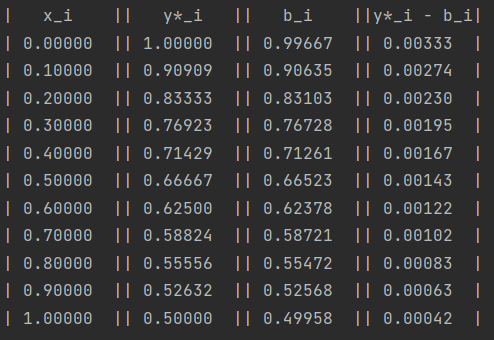
\includegraphics[width = 0.7\linewidth]{table.png}
				\end{figure}
				\pagebreak
				\begin{figure}[h]
					\centering
					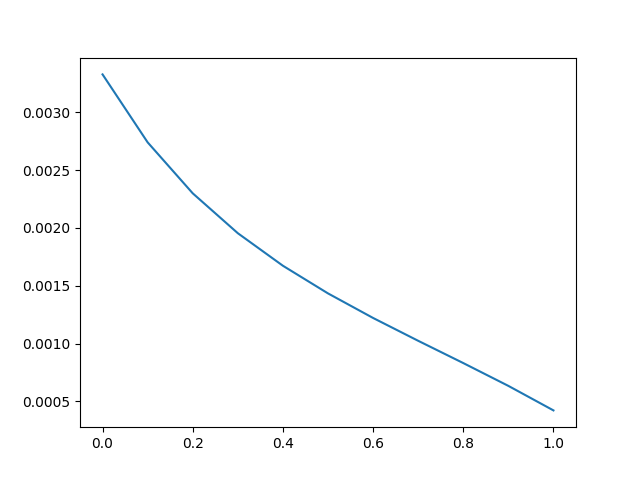
\includegraphics[width = 0.9\linewidth]{plot.png}
					\caption{График погрешности}
				\end{figure}
\end{document}	